\input{../header.tex}

\setlength{\parindent}{0em}

\begin{document}

\subsection{Implementation}
For the implementation of the \textit{MNIST} Diffusion network, the 'Denoising-Diffusion Pytorch' library ('https://github.com/lucidrains/denoising-diffusion-pytorch') was used.
It provides a predefined \textit{U-Net} architecture, where the base dimension (\texttt{DIM}) and their multiplication for every hidden layer (\texttt{DIM\_MULTS}) need to be defined.
In the case of this exercise, the amount of features of the \textit{U-Net} went from $1 \rightarrow 32 \rightarrow 64 \rightarrow 160$ for the Downsampling and $160 \rightarrow 64 \rightarrow 32 \rightarrow 1$ for the Upsampling.
Besides the entire \textit{U-Net} architecture, an additional class \texttt{diffusion} was given, containing the entire \textbf{Training} and \textbf{Sampling} algorithm, making the framework of the training and validation more compact than in the \textit{Simple Diffusion} exercise.

For the dataset and training I used the following parameters: \texttt{num\_epochs} = 100 (not used due to the huge computational cost), \texttt{learning\_rate} = $0.0004$ and \texttt{batch\_size} = 128.
Additional parameters for the \textit{U-Net} architecture and \texttt{diffusion} class were given with:
\begin{itemize}
  \item \texttt{IMAGE\_SIZE} = 28\\
  describing the amount of pixels per row/column in the \textit{MNIST} dataset 
  \item \texttt{TIME\_STEPS} = 1000\\
  The amount of time steps in the algorithm for the training
  \item \texttt{SAMPLING\_TIMESTEPS}\\
  The amount of time steps in the algorithm for the sampling
  \item \texttt{DIM} = 32 and \texttt{DIM\_MULTS} = (1, 2, 5)
\end{itemize}

\subsection{Results}
For reasons discussed in \autoref{subsec:Problems} only 20 epochs could be trained. In the loss curves (plotted within the .ipynb-file) a steady decrease is visible for the training as well as the validation.
This indicates, that the training network becomes better at predicting the added noise, which again leads to better generated \textit{MNIST} numbers.

The loss is again calculated via the Mean Squared Error (MSE) via
$$
\nonumber
\text{loss} = \text{MSE} = \frac{1}{N} \sum_{i=1}^{N}\left(\epsilon - \epsilon_\theta\right)^2
$$
with $\epsilon$ being the true value and $\epsilon_\theta$ as the prediction from the \textit{U-Net}.\\

In the following are the sampled numbers visualized for the untrained network (0th epoch) and for every fifth epoch. (With just four examples, since even the sampling took a relatively long time.) 

\begin{figure}[H]
  \centering
  \begin{subfigure}[b]{0.32\textwidth}
    \centering
    
\includegraphics[scale=0.95]{images/epoch_0.png}
    \caption{Generated digits after the 0th epoch.}
  \end{subfigure}
  \hfill
  \begin{subfigure}[b]{0.32\textwidth}
    \centering
    
\includegraphics[scale=0.95]{images/epoch_5.png}
    \caption{Generated digits after the 5th epoch.}
  \end{subfigure}
  \hfill
  \begin{subfigure}[b]{0.32\textwidth}
    \centering
    
\includegraphics[scale=0.95]{images/epoch_10.png}
    \caption{Generated digits after the 10th epoch.}
  \end{subfigure}
  \vspace{0.5cm}
  \begin{subfigure}[b]{0.48\textwidth}
    \centering
    
\includegraphics[scale=0.95]{images/epoch_15.png}
    \caption{Generated digits after the 15th epoch.}
  \end{subfigure}
  \hfill
  \begin{subfigure}[b]{0.48\textwidth}
    \centering
    
\includegraphics[scale=0.95]{images/epoch_20.png}
    \caption{Generated digits after the 20th epoch.}
  \end{subfigure}
\end{figure}

It is directly visible, that the quality of the numbers improved, since after the 10th epoch, the numbers are already recognizable.
They are still slightly improving (for example the fourth number in the 10th epoch still being undefined between a '2' and a '9') with further epochs.

In the following are the generated numbers for the \textit{GAN} training in order to compare them directly with the new \textit{diffusion} model.
\begin{figure}[H]
  \begin{subfigure}[b]{0.48\textwidth}
    \centering
    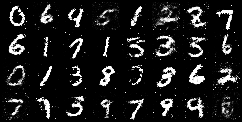
\includegraphics[scale=0.75]{../GAN/images/fake/fake_epoch_20.png}
    \caption{Generated digits (GAN) after the 20th epoch.}
  \end{subfigure}
  \hfill
  \begin{subfigure}[b]{0.48\textwidth}
    \centering
    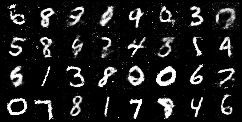
\includegraphics[scale=0.75]{../GAN/images/fake/fake_epoch_99.png}
    \caption{Generated digits (GAN) after the 99th epoch.}
  \end{subfigure}
\end{figure}

The direct comparison shows, that the numbers are generated in a higher quality and faster (in less epochs, not necessarily faster with respect to computation time) with the new \textit{diffusion} model.
After 20 epochs, the \textit{GAN} generated numbers are still mainly unrecognizable and dominated by noise. 
Only after the 99th epoch (the last one in the training) the numbers come close to the quality of the \textit{diffusion} model, but not entirely reaching it.

This indicates, that the \textit{diffusion} model generates visually more realistic numbers than the \textit{GAN} model with the given training parameters. The main question is whether the high computation cost is worth the advantages of the \textit{diffusion} models.
These are mainly the scalability, parallelization and a stable convergence, which is not guaranteed by the \textit{GAN} model.

\subsection{Problems and Improvements}
\label{subsec:Problems}
The main problem for the training is definitely the immense computational cost required for this dataset.
One epoch took approximately $\qty{15}{\minute}$, which resulted in a training of roughly $\qty{5.75}{\hour}$ for mere 20 epochs. 
While the improvement in the loss and the quality of the images are visible, the convergence was not entirely met.
A longer training was considered, but had to be canceled due to time and especially cooling problems. The used laptop only enables CPU-based training, which is extremely slow and generates a lot of heat.
For the last few epochs additional ice packs had to be used to prevent the device from overheating.
Therefore, the biggest improvement is by far the use of better hardware. 

Since most of the code was used from a library (the entire \textit{U-Net}, training and sampling), an improvement could only be made via their parameters. 
But since changing them (e.g. additional and deeper hidden layers) could also increase the computation time even further without an improvement, this idea was discarded.

The last possible improvement is again an adaptive \texttt{learning\_rate} and a hyperparameter optimization, for which the hardware is simply not good enough.

\end{document}


